\documentclass[10pt,a4paper]{article}
%\usepackage[left=4cm,right=4cm,top=3cm,bottom=3cm]{geometry}
\usepackage[utf8]{inputenc}
\usepackage[francais]{babel}
\usepackage[T1]{fontenc}
\usepackage{amsmath}
\usepackage{amsfonts}
\usepackage{amssymb}
\usepackage{graphicx}
\usepackage{color}
%\usepackage{hyperref}
\author{Abdelaziz KHALED}
\title{Les modèles d'attaquant}
\renewcommand{\thesection}{\arabic{section}}

\newcommand{\rouge}[1]{{\color{red}#1}}
\newcommand{\VERT}[1]{{\color{green}#1}}
\newcommand{\bleu}[1]{\textcolor{black}{$#1$}}
\newcommand{\bl}[1]{\textcolor{black}{#1}}
\newcommand{\Ra}{\ensuremath{\Rightarrow}}
\newcommand{\ra}{\ensuremath{\rightarrow}}
\newcommand{\RaE}{\VERT{\Ra E}}
\newcommand{\RaI}{\VERT{\Ra I}}
\newcommand{\et}{\mathop{\&}}
 \newcommand{\infer}[2]{
 \begin{array}{c}
   #1\\
   \hline \noalign{\vskip 1pt}#2
  \end{array}}
\newcommand{\inferThreeLabel}[5]{\bl{
\begin{array}{cc}
 {\VERT{#1}} \quad 
 \begin{array}{c}
   #2 \hspace{2em} #3\hspace{2em} #4\\
   \hline \noalign{\vskip 1pt}#5
  \end{array}
\end{array}}}

\newcommand{\inferTwoLabel}[4]{\bl{
\begin{array}{cc}
 {\VERT{#1}} \quad 
 \begin{array}{c}
   #2 \hspace{2em} #3\\
   \hline \noalign{\vskip 1pt}#4
  \end{array}
\end{array}}}

\newcommand{\leafLabel}[2]{\bl{
 {\VERT{#1}} \quad
  \begin{array}{c}
  #2
  \end{array} }}

\newcommand{\inferLabel}[3]{\bl{
    \begin{array}{cc}
    {\VERT{#1}} \quad
    \begin{array}{c}
      #2\\
      \hline \noalign{\vskip 1pt}#3
    \end{array}
  \end{array}
  }}

    
\newcommand{\heading}[1]{%      % ca c'est des commandes a moi
  \begin{center}                % mais ca peut t'interesser
    \large\bf
    \color{cyan}{\shadowbox{#1}}%
  \end{center}
  \markright{#1}
  \vspace{1ex minus 1ex}}

\newcommand{\subheading}[1]{%
  \begin{center}
    \color{green}{\bf\Ovalbox{#1}}
  \end{center}}

\begin{document}
\let\cleardoublepage\clearpage
\maketitle
\newpage
\tableofcontents
\newpage
\section{Introduction}
Depuis l’attaque d’un site de production d’uranium en 2010 (le Vers Stuxnet), le nombre
de cyber attaques de systèmes de contrôle de production industrielle n’a cessé d’augmenter.\newline
 
D'une part, l'évolution des technologies amène les systèmes de pilotage informatisé des installations à s'ouvrir aux réseaux extérieurs, ce qui génère une augmentation des risques.\newline

D’autre part, les composants techniques utilisés dans les systèmes de contrôle industriel sont en général peu préparés aux défis de la sécurité informatique.
\newline

Notre objectif est de créer un framework qui permet de générer automatiquement les scénarios d'attaques contre les systèmes industriels à partir des différentes configurations et différents modèles d'attaquant. Dans la première étape on spécifie un modèle du système(agents, canaux et protocoles de communication, messages, etc.) ainsi que les propriétés de sécurité attendues et les différents modèles d'attaquant spécifiques envisagés. La deuxième étape on utilise le modèle checking UPPAAL pour produire les scénarios d'attaques.\newline
  
Nous présentons dans ce rapport les différents modèles d'attaquant et leurs modélisations avec le model checking UPPAAL.  
\section{Modèles d'attaquant}
L'attaquant est l'entité principale dans la vérification des protocoles cryptographiques et la génération des scénarios d'attaques. Dans~\cite{ref1}, les auteurs ont classé les attaquants en plusieurs classes. Dans notre travail on a regroupé les attaquants en deux classes : \textit{les attaquants externes} et \textit{les attaquants internes}. L'attaquant externe est celui qui peut écouter de façon passive le réseau, forger, modifier ou rejouer les messages entre les agents. L'attaquant interne dispose de plus de capacités. Il peut jouer le rôle d'un ou plusieurs agent(s) légitime(s).\newline

La formalisation des attaquants peut \^{e}tre basé sur des processus comme CSP~\cite{ref6} et SPi-calcul\cite{ref7}, des logique comme les clauses de Horn~\cite{ref2} ou encore les règles de réécriture.\newline  

Dans cette partie on va présenter la formalisation de différents modèles d'attaquant avec les clauses de Horn.   
% parler sur les défférents classe des attaquants qui existe et ce quoi les classes qui on va utilisé 
\subsection{Clauses de Horn}
\paragraph{}
Une $clause\; de\; Horn$ est une disjonction de littéraux, c'est-à-dire une clause comportant au plus un littéral positif.  
\[(A_{1}\wedge...\wedge A_{n})\Rightarrow B ,\;\;\;\; avec\;\; n \in N  \]
$A_{i}$ et $B$ sont des atomes de la forme $P(t_{1},...,t_{k})$,où $P$ est un prédicat k-aires et $t_{i}$ sont des termes. $B$ est appelé la t\^{e}te de clause et $A_{1}\wedge...\wedge A_{n}$ le corps de la clause. Une clause unité (ou fait) est une clause de Horn dont le corps est vide, c'est-à-dire comportent un littéral positif et aucun littéral négatif.\newline

Un but est une clause de Horn dont la t\^{e}te est vide, c'est-à-dire ne contenant aucun littéral positif. 		    \newline

L'idée principale de formalisation avec les clauses de Horn~\cite{ref2} est l’utilisation des
termes pour représenter les messages et les prédicats pour indiquer qu'un terme est connu de l'attaquant, exemple: \textit{attaquant(m)} indique que l'attaquant peut avoir le terme $m$   (message). Dans la \textit{section 2.3} on explique comment formaliser les attaquants avec les clauses de Horn.

\subsection{Le Modèle Dolev-Yao}
Le modèle de l'attaquant le plus courant est celui de Dolev-Yao~\cite{ref3}. Il a un contr\^{o}le complet sur le réseau et il peut dériver de nouveaux messages à partir de ses connaissances initiales et les messages reçus de la part des agents légitimes. Pour obtenir un nouveau message, l'attaquant peut composer et décomposer, chiffrer et déchiffrer des messages, dans le cas o\`{u} il connaît la clé.\newline

Notons que la connaissance initiale d’un attaquant se limite aux clés publiques de tous les agents, à sa clé privée. Ci-dessous, les règles de déduction de l'attaquant Dolev-Yao :\newline
\begin{center}
\begin{tabular}{|l|c|}
  \hline
  $\inferLabel{}{ u \in I}{I\vdash u}$ & Capacité à reconnaitre un terme \\
  \hline
  $\inferLabel{}{ I \vdash \langle u,v \rangle}{I\vdash u}$ & Capacité à décomposer un message  \\
  \hline
  $\inferLabel{}{ I \vdash \langle u,v \rangle}{I\vdash v}$ & Capacité à décomposer un message \\
  \hline
  $\inferLabel{}{ I \vdash u \hspace{5pt} I \vdash v }{I \vdash \langle u,v \rangle}$ & Capacité  à  composer  un  terme  à  partir  de  deux termes \\
  \hline
  $\inferLabel{}{ I \vdash u \hspace{5pt} I \vdash v }{I \vdash {\lbrace u \rbrace}_{v}}$ & Capacité  à  chiffrer  un  message  avec  une  clé connue \\
  \hline
  $\inferLabel{}{ I \vdash {\lbrace u \rbrace}_{v} \hspace{5pt} I \vdash v }{I \vdash u}$ & Capacité  à  déchiffrer  un  message  avec  une  clé connue \\
  \hline
    $\inferLabel{}{ I \vdash u }{I \vdash H|u|}$ & Capacité  à  hacher un message \\
  \hline
\end{tabular}
\end{center}
\medskip

\paragraph{}
La notation $I \vdash u$ signifie que l’attaquant à partir de ses connaissances courantes $I$,
est capable de déduire $u$ grâce à son système de déduction.
  
\subsection{Formalisation de différents modèles d'attaquant}
Les primitives cryptographiques sont représentées par des prédicats. Pour le chiffrement on utilise ${\lbrace m\rbrace}_{pub(k)}$ , le hachage est présenté par $H|m|$ et la signature par ${\lbrace H|m|\rbrace}_{priv(k)}$. Ci-dessous, la représentation des prédicats :\newpage
  
\begin{equation}
attaquant(m)\wedge attaquant(pub(k))\Longrightarrow attaquant({\lbrace m\rbrace}_{pub(k)})
\end{equation}
\begin{equation}
attaquant({\lbrace m\rbrace}_{pub(k)}) \wedge attaquant(priv(k))\Longrightarrow attaquant(m) 
\end{equation}
\begin{equation}
attaquant(m)\wedge attaquant(priv(k))\Longrightarrow attaquant({\lbrace H|m|\rbrace}_{priv(k)})
\end{equation}
$(1)$ l'attaquant peut chiffrer, $(2)$ déchiffrer avec la clé privée, $(3)$ signer un message.\newline

Pour l'envoi ou la réception des messages on utilise le prédicat $canal(c,m)$, signifié que le message $m$ est envoyé sur le canal $c$.  
\begin{equation}
canal(c,m)\wedge attaquant(c)\Longrightarrow attaquant(m)
\end{equation}
\begin{equation}
attaquant(m)\wedge attaquant(c)\Longrightarrow canal(c,m) 
\end{equation}
$(4)$ l'attaquant peut recevoir le message, $(5)$ l'attaquant peut envoyer le message.\newline

Pour forger un nouveau message l'attaquant peut composer, décomposer, chiffrer et déchiffrer les messages.
\begin{equation}
attaquant(m_{1})\wedge attaquant(m_{2})\Longrightarrow attaquant(\langle m_{1},m_{2}\rangle) 
\end{equation}
\begin{equation}
attaquant(\langle m_{1},m_{2}\rangle)\Longrightarrow attaquant(m_{1}) 
\end{equation}
\begin{equation}
attaquant(\langle m_{1},m_{2}\rangle)\Longrightarrow attaquant(m_{2}) 
\end{equation}
$(6)$ l'attaquant peut composer un message, $(7)(8)$ l'attaquant peut décomposer un message.\newline 

Pour modifier un message on utilise les prédicats $(9)(10)$.\newline
\begin{equation}
attaquant(\langle m_{1},m_{2}\rangle)\wedge attaquant(m_{3})\Longrightarrow attaquant(\langle m_{1},m_{3}\rangle) 
\end{equation}
\begin{equation}
attaquant(\langle m_{1},m_{2}\rangle)\wedge attaquant(m_{3})\Longrightarrow attaquant(\langle m_{3},m_{2}\rangle) 
\end{equation}

Pour rejouer un message l'attaquant d'abord doit copier le message dans la base de connaissances et aprés il peut rejouer le message.
\begin{equation}
canal(c,m)\wedge attaquant(c)\Longrightarrow attaquant(copier(m))
\end{equation}
\begin{equation}
attaquant(selection(m))\wedge attaquant(c)\Longrightarrow canal(c,m) 
\end{equation}

Pour bloquer un message l’attaquant intercepte le message sur le canal $c_{1}$ et le redirige vers canal $c_{2}$
\begin{equation}
canal(c_{1},m)\wedge attaquant(c_{1})\Longrightarrow attaquant(m)
\end{equation}
\begin{equation}
attaquant(m)\wedge attaquant(c_{2})\Longrightarrow canal(c_{2},m) 
\end{equation}

\subsubsection{Attaquant 1 :}
Cet attaquant est basé sur le modèle Dolev-Yao, peut :
\begin{itemize}
\item intercepter les messages.
\item chiffrer, déchiffrer ou signer les messages.
\item bloquer les messages.
\item copier les messages.
\item modifier, forger ou rejouer les messages.\\
\end{itemize}
Formalisation de l'attaquant :   
\[
\begin{array}{l}
canal(c,m)\wedge attaquant(c)\Longrightarrow attaquant(m)\\
attaquant(m)\wedge attaquant(c)\Longrightarrow canal(c,m)\\
attaquant(m)\wedge attaquant(pub(k))\Longrightarrow attaquant({\lbrace m\rbrace}_{pub(k)})
\\
attaquant({\lbrace m\rbrace}_{pub(k)}) \wedge attaquant(priv(k))\Longrightarrow attaquant(m) 
\\ 
attaquant(m)\wedge attaquant(priv(k))\Longrightarrow attaquant({\lbrace H|m|\rbrace}_{priv(k)})
\\
attaquant(m_{1})\wedge attaquant(m_{2})\Longrightarrow attaquant(\langle m_{1},m_{2}\rangle)\\ 
attaquant(\langle m_{1},m_{2}\rangle)\Longrightarrow attaquant(m_{1})\\ 
attaquant(\langle m_{1},m_{2}\rangle)\Longrightarrow attaquant(m_{2})\\ 
attaquant(\langle m_{1},m_{2}\rangle)\wedge attaquant(m_{3})\Longrightarrow attaquant(\langle m_{1},m_{3}\rangle)\\ 
attaquant(\langle m_{1},m_{2}\rangle)\wedge attaquant(m_{3})\Longrightarrow attaquant(\langle m_{3},m_{2}\rangle)\\ 
canal(c,m)\wedge attaquant(c)\Longrightarrow attaquant(copier(m))\\
attaquant(selection(m))\wedge attaquant(c)\Longrightarrow canal(c,m)\\ 
canal(c_{1},m)\wedge attaquant(c_{1})\Longrightarrow attaquant(m)\\
attaquant(m)\wedge attaquant(c_{2})\Longrightarrow canal(c_{2},m)\\ 
\end{array}
\]
\subsubsection{Attaquant 2 :}
Le rôle principal de cet attaquant est modifié les messages. Il peut :
\begin{itemize}
\item intercepter les messages.
\item chiffrer, déchiffrer ou signer les messages.
\item Modifier le message complet ou juste un champ.\\
\end{itemize}
Formalisation de l'attaquant :   
\[
\begin{array}{l}
canal(c,m)\wedge attaquant(c)\Longrightarrow attaquant(m)\\
attaquant(m)\wedge attaquant(c)\Longrightarrow canal(c,m)\\
attaquant(m)\wedge attaquant(pub(k))\Longrightarrow attaquant({\lbrace m\rbrace}_{pub(k)})
\\
attaquant({\lbrace m\rbrace}_{pub(k)}) \wedge attaquant(priv(k))\Longrightarrow attaquant(m) 
\\ 
attaquant(m)\wedge attaquant(priv(k))\Longrightarrow attaquant({\lbrace H|m|\rbrace}_{priv(k)})
\\
attaquant(\langle m_{1},m_{2}\rangle)\wedge attaquant(m_{3})\Longrightarrow attaquant(\langle m_{1},m_{3}\rangle)\\ 
attaquant(\langle m_{1},m_{2}\rangle)\wedge attaquant(m_{3})\Longrightarrow attaquant(\langle m_{3},m_{2}\rangle)\\ 
  
  \end{array}
\]

\subsubsection{Attaquant 3 :}
Le rôle principal de cet attaquant est forger les messages. Il peut :
\begin{itemize}
\item chiffrer, déchiffrer ou signer les messages.
\item forger les messages.\\
\end{itemize}
Formalisation de l'attaquant :   
\[
\begin{array}{l}
attaquant(m)\wedge attaquant(pub(k))\Longrightarrow attaquant({\lbrace m\rbrace}_{pub(k)})
\\
attaquant({\lbrace m\rbrace}_{pub(k)}) \wedge attaquant(priv(k))\Longrightarrow attaquant(m) 
\\ 
attaquant(m)\wedge attaquant(priv(k))\Longrightarrow attaquant({\lbrace H|m|\rbrace}_{priv(k)})
\\
attaquant(m_{1})\wedge attaquant(m_{2})\Longrightarrow attaquant(\langle m_{1},m_{2}\rangle)\\ 
attaquant(\langle m_{1},m_{2}\rangle)\Longrightarrow attaquant(m_{1})\\ 
attaquant(\langle m_{1},m_{2}\rangle)\Longrightarrow attaquant(m_{2})\\ 
attaquant(m)\wedge attaquant(c)\Longrightarrow canal(c,m)\\
 
  \end{array}
\]

\subsubsection{Attaquant 4 :}
Le rôle principal de cet attaquant est rejoué les messages. Il peut :
\begin{itemize}
\item intercepter les messages.
\item copier les messages.
\item rejouer les messages.\\
\end{itemize}
Formalisation de l'attaquant :   
\[
\begin{array}{l}
canal(c,m)\wedge attaquant(c)\Longrightarrow attaquant(copier(m))\\
attaquant(selection(m))\wedge attaquant(c)\Longrightarrow canal(c,m) 
  
  \end{array}
\]

\subsubsection{Attaquant 5 :}
Le rôle principal de cet attaquant est bloqué ou retardé les messages. Il peut :
\begin{itemize}
\item intercepter les messages.
\item bloquer les messages.
\item retarder les messages.\\
\end{itemize}
Formalisation de l'attaquant :   
\[
\begin{array}{l}
canal(c_{1},m)\wedge attaquant(c_{1})\Longrightarrow attaquant(m)\\
attaquant(m)\wedge attaquant(c_{2})\Longrightarrow canal(c_{2},m) 
\end{array}
\]

\section{Modèles d'attaquant avec UPPAAL}
UPPAAl~\cite{ref4} est une bo\^{i}te à outils a été développé conjointement par l'université d'Aalborg et l'université d'Uppsala. Il permet de vérifier des réseaux d'automates temporisés. Les propriétés qui peuvent \^{e}tre vérifiées sont principalement des propriétés d'accessibilité, de sûreté, de vivacité ou d'états bloquants. La logique utilisée par UPPAAL est un fragment de TCTL qui n'autorise pas les embo\^{i}tements d'opérateurs temporels. L'algorithme implémenté dans UPPAAL est un algorithme d'analyse en avant.
   
\subsection{Le modèle UPPAAL}
Le modèle qui peut-\^{e}tre vérifié par UPPAAL est une variante des automates temporisés. Ce modèle permet de représenter des contraintes d'urgence(une transition doit \^{e}tre prise immédiatement), des contraintes d'atomicité(une séquence de transitions doit \^{e}tre franchie instantanément). Un automate temporisé est défini comme suit~\cite{ref5} :
\paragraph{Définition :}
Un automate temporisé $A$ est un tuple $\langle N, l_{0}, C, E, I, \Sigma \rangle$ o\`{u} :
\begin{itemize}
\item $N$ est un ensemble fini d'états,
\item $l_{0} \in N$ est l'état initiale,
\item $C$ un ensemble fini d'horloges,
\item $E \subseteq N \times B(C) \times \Sigma \times 2^c \times N$ est un ensemble fini de transitions, 
\item $I : N \longrightarrow B(c)$ associe un invariant à chaque état,
\item $\Sigma$ est un alphabet d'action.\newline
\end{itemize}

Un état de l'automate peut comporter une condition sur les horloges $B(c)$, appelés $invariant$, qui doit \^{e}tre satisfaite pour passer vers l'état suivant. Une transition de l'automate est étiquetée par:
\begin{itemize}
\item une $garde$, qui exprime une condition sur les valeurs des variables, elle doit \^{e}tre satisfaite pour franchir la transition.
\item une $synchronisation$ de la forme $c!$ pour l'émission de signal ou $c?$ pour la réception de signal.
\item une remise à zéro pour certaines horloges et une mise à jour de certaines variables.
\end{itemize}

\subsection{La modélisation de différents modèles d'attaquant}
Les primitives cryptographiques sont représentées par un automate $SecureData$, qui permet de chiffrer, déchiffrer, signer ou vérifier la signature. La figure ci-dessous, représente l'automate $SecureData$ :
\begin{figure}[!h]
\begin{center}
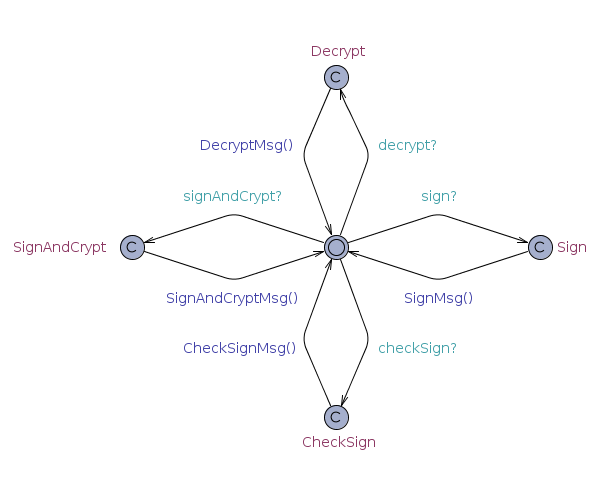
\includegraphics[scale=0.5]{img/secureData.png}\newline
\caption{Automate SecureData}
\end{center}
\end{figure}

Pour chiffrer un message, on doit calculer $m+2p$ , $m$ c'est le message et $p$ représente la clé publique. Le déchiffrement s'effectue avec $m-s$ , $s$ représente la clé privée et $s=2p$. Les agents de réseaux peuvent utiliser cet automate à l'aide des canaux de communication $sign$, $signAndCrypt$, $decrypt$ et $checkSign$.
\subsubsection{Attaquant 1 :}
La figure 2 représente un attaquant qui fonctionne comme \textit{Dolev-Yao}. Il peut recevoir et envoyer les messages à travers le canal $c2s$. La variable locale $i$ borne le nombre total d'actions autorisées à faire à chaque tour. Si l'attaquant déplace à l'état $I1$, il peut décider de faire les actions citées dans la \textit{section 2.3.1}.
      
\begin{figure}[!h]
\centering 
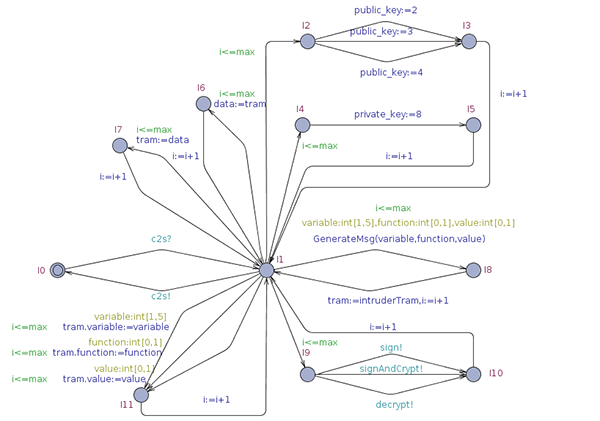
\includegraphics[scale=0.5]{img/attaquant1-600.png}
\caption{Automate de l'attaquant 1}
\end{figure}

\subsubsection{Attaquant 2 :}
Le rôle principal de cet attaquant est modifié une partie du message ou le message complet à partir des connaissances de l'attaquant. Si l'attaquant déplace à l'état $I1$, il peut décider de faire les actions citées dans la \textit{section 2.3.2}. La figure ci-dessous, représente l'automate de l'attaquant 2:  

\begin{figure}[!h]
\centering 
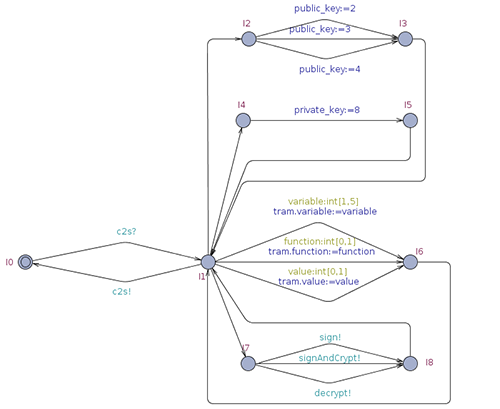
\includegraphics[scale=0.5]{img/attaquant2-500.png}
\caption{Automate de l'attaquant 2}
\end{figure}
\newpage
\subsubsection{Attaquant 3 :}
Le rôle principal de cet attaquant est forger les messages par force brute à partir des connaissances de l'attaquant. Si l'attaquant déplace à l'état $I1$, il peut décider de faire les actions citées dans la \textit{section 2.3.3}. La figure ci-dessous, représente l'automate de l'attaquant 3:  

\begin{figure}[!h]
\centering 
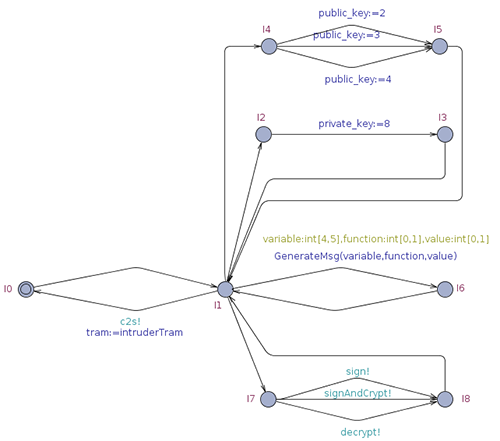
\includegraphics[scale=0.5]{img/attaquant3-500.png}
\caption{Automate de l'attaquant 3}
\end{figure}

\subsubsection{Attaquant 4 :}
Le rôle principal de cet attaquant est rejouer les messages. Pour rejouer les messages l'attaquant peut copier un seul message dans la variable $data$ et après il peut l'utiliser pour changer le message $tram$. La figure ci-dessous, représente l'automate de l'attaquant 4:  

\begin{figure}[!h]
\centering 
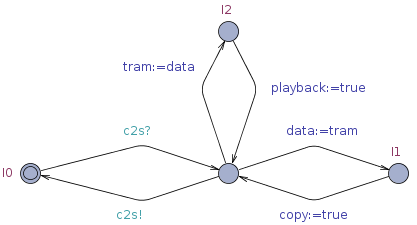
\includegraphics[scale=0.6]{img/attaquant4.png}
\caption{Automate de l'attaquant 4}
\end{figure}

\subsubsection{Attaquant 5 :}
Le rôle principal de cet attaquant est de bloquer ou retarder les messages. L'attaquant dans l'état $I1$ peut décider de retourner vers l'état $I0$ sans envoyé le message dans ce cas on a bloqué le message ou envoyer le message mais après un certain temps dans ce cas on a retardé le message. La figure ci-dessous, représente l'automate de l'attaquant 5:  

\begin{figure}[!h]
\centering 
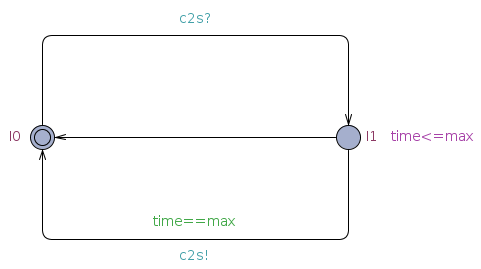
\includegraphics[scale=0.5]{img/attaquant5.png}
\caption{Automate de l'attaquant 5}
\end{figure}

\section{Comparaison entre CSP, SPi-calculus et les clauses de Horn}
Le CSP(Communicating Sequential Processes) et SPi-calculus sont suffisamment riches pour modéliser les différents modèles d'attaquant par apport à les clauses de Horn. On peut voir la différence entre les clauses d'Horn, CSP et SPi-calcul dans les points suivants :\newline

\begin{itemize}
\item La représentation de l’attaquant avec les clauses de Horn est basé sur un ensemble des prédicats, par contre avec CSP et SPi-calculus l’attaquant est représenté comme un processus.
\item Il existe un ensemble des commandes dans CSP et SPi-calculus comme : \textit{commande parallèle}, \textit{commande alternative},\textit{commande répétitive},...etc
\item CSP et SPi-calculus intègrent un mécanisme de synchronisation basé sur le principe du rendez-vous, par contre pour les clauses de Horn il faut modéliser des prédicats qui expriment l'envoi ou la réception du message.
\item Avec les clauses de Horn il faut définir des prédicats pour exprimer les primitives cryptographiques, par contre à SPi-calculus elles sont déja définies.
\end{itemize}


\section{Conclusion}
En conclusion, nous avons présenté les différents modèles d'attaquant et leurs modélisations avec le model checking UPPAAL. Cependant, au vu des résultats obtenus lors de la mise en pratique, il appara\^{i}t que ce modèle peut trouver des attaques dans un temps raisonnable.
\newpage
\bibliography{mabiblio}
\bibliographystyle{plain}

\end{document}
